\section{Operating Systems}

\subsection{Microsoft Windows}
Microsoft Windows, commonly referred to as Windows, is a family of graphical operating systems developed, marketed, and sold by Microsoft Corporation since 1985. It is designed for use on personal computers, workstations, servers, and smartphones. The name "Windows" originates from the window-based graphical user interface (GUI) known as File Explorer. Windows is a multitasking operating system, meaning it can run multiple programs simultaneously. From its inception, Windows has been conceived as a graphical operating system, implementing the "desktop metaphor" with icons, buttons, backgrounds, taskbars, status bars, and many other features.

\subsubsection{Windows Shell and PowerShell}
The shell, or command interpreter, is a program that allows interaction with the operating system via a terminal and command-line interface. Windows PowerShell is an advanced shell integrated into all Microsoft operating systems starting from Windows 7. It includes an interactive prompt and a scripting environment that can be used separately or in combination. PowerShell is a command-line shell designed specifically for system administrators, offering extensive scripting capabilities to automate routine tasks. Key features and advantages of PowerShell include:
\begin{itemize}
    \item \textbf{Integration with Microsoft .NET}: PowerShell leverages the .NET framework, providing extensive functionality through reusable libraries and functions.
    \item \textbf{Object-Oriented}: Unlike traditional shells that return plain text, PowerShell returns objects, enabling more complex data manipulation.
    \item \textbf{Command-Lets (cmdlets)}: PowerShell commands are structured as verb-noun pairs, facilitating intuitive command usage.
    \item \textbf{Admin-Oriented}: PowerShell includes features designed for system administrators, such as remote management and the ability to perform administrative tasks.
\end{itemize}

\subsubsection{Common PowerShell Cmdlets}
One of PowerShell's strengths is its cmdlets, which are structured as a verb followed by a noun. To display the complete set of available cmdlets, the \texttt{Get-Command} cmdlet can be used. PowerShell allows the use of the pipe operator (|) to chain multiple cmdlets, using the output of one cmdlet as the input for the next. This technique is particularly useful for text processing tasks.

\begin{table}[h!]
    \centering
    \begin{adjustbox}{width=1\textwidth}
    \begin{tabular}{|c|c|c|}
    \hline
    \textbf{Cmdlet} & \textbf{Aliases} & \textbf{Description} \\
    \hline
    \texttt{Set-Location} & cd, chdir, sl & Sets the current working location to a specified location. \\
    \texttt{Get-Content} & cat, gc, type & Gets the content of the item at the specified location. \\
    \texttt{Add-Content} & ac & Adds content to the specified items, such as adding words to a file. \\
    \texttt{Set-Content} & sc & Writes or replaces the content in an item with new content. \\
    \texttt{Copy-Item} & copy, cp, cpi & Copies an item from one location to another. \\
    \texttt{Remove-Item} & del, erase, rd, ri, rm, rmdir & Deletes the specified items. \\
    \texttt{Move-Item} & mi, move, mv & Moves an item from one location to another. \\
    \texttt{Set-Item} & si & Changes the value of an item to the value specified in the command. \\
    \texttt{New-Item} & ni & Creates a new item. \\
    \texttt{Start-Job} & sajb & Starts a Windows PowerShell background job. \\
    \texttt{Compare-Object} & compare, dif & Compares two sets of objects. \\
    \texttt{Group-Object} & group & Groups objects that contain the same value for specified properties. \\
    \hline
    \end{tabular}
\end{adjustbox}
    \caption{Common PowerShell Cmdlets}
    \label{table:cmdlets}
    \end{table}

    \begin{table}[h!]
    \centering
    \begin{adjustbox}{width=1\textwidth}
    \begin{tabular}{|c|c|c|}
    \hline
    \textbf{Cmdlet} & \textbf{Aliases} & \textbf{Description} \\
    \hline
    \texttt{Invoke-WebRequest} & curl, iwr, wget & Gets content from a web page on the Internet. \\
    \texttt{Measure-Object} & measure & Calculates numeric properties of objects, and the characters, words, and lines in string objects. \\
    \texttt{Resolve-Path} & rvpa & Resolves the wildcard characters in a path and displays the path contents. \\
    \texttt{Resume-Job} & rujb & Restarts a suspended job. \\
    \texttt{Set-Variable} & set, sv & Sets the value of a variable. Creates the variable if one with the requested name does not exist. \\
    \texttt{Show-Command} & shcm & Creates Windows PowerShell commands in a graphical command window. \\
    \texttt{Sort-Object} & sort & Sorts objects by property values. \\
    \texttt{Start-Service} & sasv & Starts one or more stopped services. \\
    \texttt{Start-Process} & saps, start & Starts one or more processes on the local computer. \\
    \texttt{Suspend-Job} & sujb & Temporarily stops workflow jobs. \\
    \texttt{Wait-Job} & wjb & Suppresses the command prompt until one or all of the Windows PowerShell background jobs running in the session are complete. \\
    \texttt{Where-Object} & ?, where & Selects objects from a collection based on their property values. \\
    \hline
    \end{tabular}
    \end{adjustbox}
    \caption{Additional PowerShell Cmdlets}
    \label{table:cmdlets2}
    \end{table}

\subsubsection{Windows File System}
The Windows file system is an organizational structure within the operating system that regulates the naming, storage, and retrieval of files. PowerShell provides cmdlets to interact with the file system, files, and directories.

\begin{itemize}
    \item \texttt{Get-ChildItem}: Displays the contents of a directory.
    \item \texttt{Copy-Item}: Copies a file from one location to another. This cmdlet accepts two parameters: the source file and the destination.
\end{itemize}

\subsubsection{Components of Windows Operating System}
The fundamental components of the Windows operating system are depicted in the diagram (Figure~\ref{fig:components}). Windows OS distinguishes between user space and kernel space as a security measure, separating tasks that require special privileges from those that do not. The DLL (Dynamic Link Library) subsystems interface between kernel mode and user mode, providing function libraries that users and applications can utilize to request the kernel to perform specific tasks.

\begin{figure}[h!]
\centering
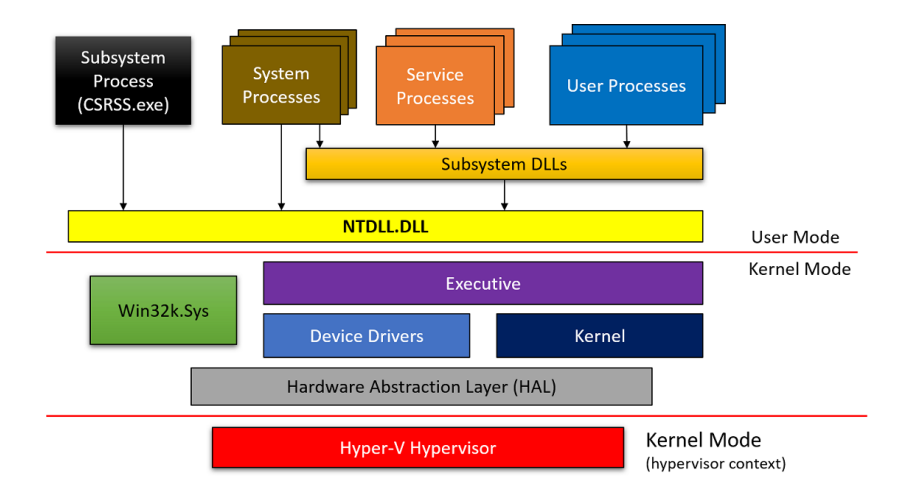
\includegraphics[width=0.8\textwidth]{images/user_kernel.png}
\caption{Components of Microsoft Windows Operating System}
\label{fig:components}
\end{figure}

\begin{itemize}
    \item User Applications: User applications run in user mode and can be either 32-bit or 64-bit, depending on the operating system.
    \item Services: This includes active processes and services in Windows, such as the task manager or network services.
    \item Executive: The executive contains the core functionalities of the operating system, including memory management, security features, and process management.
    \item Driver Management: Manages calls to input/output devices.
    \item Kernel: The kernel encompasses low-level OS functions, such as thread scheduling, interrupts, exception handling, and multiprocessor synchronization.
\end{itemize}



\subsubsection{Windows Hybrid Kernel}
The Windows kernel is a hybrid kernel, meaning it incorporates elements of both monolithic and microkernel architectures.

\begin{itemize}
    \item Monolithic Kernel: A monolithic kernel runs most operations directly in kernel space, including memory management, process management, and system calls, providing high performance but potentially lower stability due to the lack of isolation between components.
    \item Microkernel: A microkernel, conversely, delegates many functionalities to user space processes, keeping only essential functions in the kernel, which enhances modularity and stability at the cost of potential performance overhead due to increased inter-process communication.
    \item Hybrid Kernel: Windows hybrid kernel aims to balance the speed of a monolithic kernel with the modularity and stability of a microkernel by implementing critical functions within the kernel and allowing certain components, such as device drivers, to run in user space.
\end{itemize}


\subsection{Linux Operating Systems}
The origins of the Unix Operating System date back to the late 1960s with the development of the MULTICS (Multiplexed Information and Computing Service) project. This project was a collaboration between AT\&T, Honeywell, General Electric, and the Massachusetts Institute of Technology (MIT), sponsored by ARPA, the research arm of the U.S. Department of Defense. The goal was to create an operating system capable of continuing to function even if some parts of the computer were shut down or deactivated, thereby not affecting the work of users utilizing the still-active components. The modularity of this system allowed for improvements or expansions by simply adding new modules, without the need to rebuild the entire system from scratch.

In 1991, Linus Torvalds, a computer science student from Helsinki, released a version of the Minix monolithic kernel that could run on a standard Intel 386 processor, and he distributed it freely along with its source code. This project evolved into what we now know as the Linux kernel, which has been periodically updated and revised over the years.

Today, Linux is one of the most widely used operating systems for:
\begin{itemize}
    \item Web Servers
    \item High-performance applications
    \item Embedded systems
    \item Network systems
\end{itemize}
Linux is freely distributed, meaning that all users can download it and contribute to the project. The term "free software" was initially popularized by Richard Stallman, emphasizing that users are granted the following rights:
\begin{itemize}
    \item The freedom to run the program
    \item The freedom to study how the program works
    \item The freedom to redistribute copies of the program
    \item The freedom to modify the program
\end{itemize}

\subsubsection{Structure of the Linux Operating System}
As an operating system, Linux serves as an interface between the user and the machine, providing a set of tools and functionalities. The primary components are:
\begin{itemize}
    \item Hardware
    \item Operating System
    \item Shell
    \item GUI (Graphical User Interface)
    \item Applications
\end{itemize}
The operating system sits between the hardware and user applications, providing routines for managing processes, memory, and other resources. This type of kernel is known as a "monolithic" kernel.

\subsubsection{Types of Kernels}
There are several types of kernels used in operating systems:
\begin{itemize}
    \item \textbf{Microkernel}: A minimalistic kernel that includes only the basic functionalities required for the operating system to function. An example is MINIX.
    \item \textbf{Monolithic Kernel}: A single binary file that includes most of the operating system's functionalities. An example is the Unix kernel.
    \item \textbf{Modular Kernel}: An extension of the monolithic kernel, capable of adding or removing modules as needed.
\end{itemize}

\begin{figure}[h!]
\centering
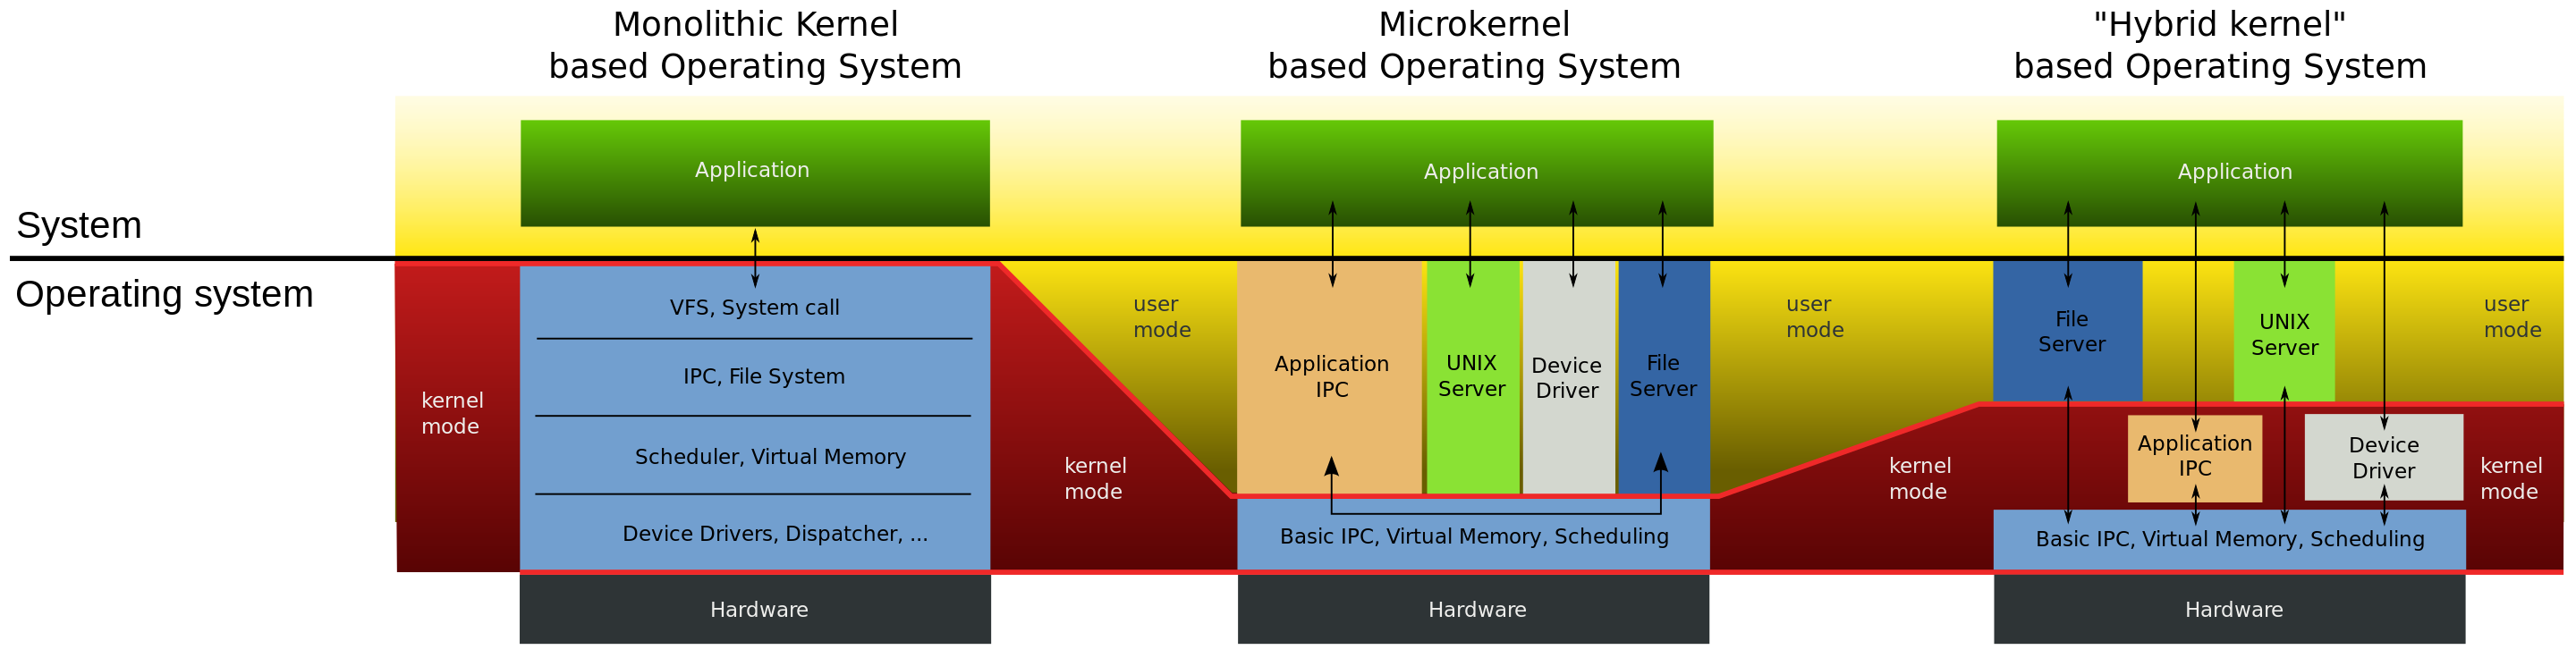
\includegraphics[width=\textwidth]{images/kernels.png}
\caption{Types of Kernels: Microkernel, Modular, Monolithic}
\label{fig:kernels}
\end{figure}

\subsubsection{Processes in Linux}
In Linux, a process is an instance of a program in execution, assigned to a processor for instruction execution. A process has a state, which is read by the CPU for scheduling and process switching. Linux processes are complex structures characterized by:
\begin{itemize}
    \item Memory addresses used
    \item Content of the addressed memory
    \item Pointers to input/output devices used
    \item Data, i.e., variables used by the process
    \item Threads
\end{itemize}

\paragraph{Threads}
Threads are tasks within a process. A process can perform various functions using multiple threads, each handling separate tasks. Threads within a process share the same state and memory information, allowing independent action on the used resources. Proper prioritization by the operating system is crucial to avoid simultaneous modification of the same resource by different threads (synchronization issue).

In Linux, each process is identified by a Process Identifier (PID), while each thread within a process is identified by a Thread Identifier (TID). Processes are created by invoking the system call \texttt{Fork()}. The child process created with \texttt{Fork()} inherits attributes from the parent process.

\begin{table}[h!]
\centering
\begin{tabular}{|c|c|}
\hline
\textbf{Command} & \textbf{Description} \\
\hline
\texttt{mkdir} & Creates a directory \\
\texttt{rmdir} & Removes a directory \\
\texttt{cp} & Copies files and directories \\
\texttt{rm} & Removes files \\
\texttt{mv} & Moves or renames files \\
\texttt{ls} & Lists directory contents \\
\texttt{cd} & Changes the current directory \\
\hline
\end{tabular}
\caption{Common Linux File System Commands}
\label{table:filesystem_commands}
\end{table}

\subsubsection{Linux File System}
The Linux file system originates in the root directory, denoted as \texttt{/}. The root user, or system administrator, has extensive control over the system. Key directories in the Linux file system include:
\begin{itemize}
    \item \texttt{/bin}: Contains essential system programs available for booting the system.
    \item \texttt{/home}: Contains user-specific directories and files.
    \item \texttt{/usr}: Contains installed programs, manual files, and documentation.
    \item \texttt{/sbin}: Similar to \texttt{/bin} but for system administration.
    \item \texttt{/etc}: Contains system and application configuration files.
\end{itemize}

\subsubsection{User Management in Linux}
Linux systems often support multiple users, necessitating mechanisms to separate user data and protect privacy. Each user is assigned a unique user identifier (UID) and a home directory. File permissions ensure that private files are not accessible to other users. User information is stored in \texttt{/etc/passwd}, which includes:
\begin{itemize}
    \item Group IDs
    \item User IDs
    \item Login shell
    \item Encrypted password (hashed)
\end{itemize}

Linux, with its rich history and robust architecture, continues to be a cornerstone in modern computing. Its versatility, security, and open-source nature make it a preferred choice for servers, high-performance applications, embedded systems, and network systems.
